\chapter{Θεωρητικό υπόβαθρο}
\label{ch:theoreteical_background}

\section{Νευρωνικά δίκτυα}
Το νευρωνικό δίκτυο με την αφηρημένη έννοια του είναι μια δομή η οποία θα μπορούσε να χαρακτηριστεί ως ένας μηχανισμός αριθμητικών πράξεων με συνήθως περισσότερες από μια εισόδους και μια ή περισσότερες εξόδους. Ένα νευρωνικό δίκτυο αποτελείται από τους κόμβους--νευρώνες του (\tl{\textbf{nodes}}) οι οποίοι ενώνονται μέσω των συνάψεων του. Το σύνολο των κόμβων οι οποίοι συνδέονται με τις ίδιες ομάδες συνάψεων λέγεται επίπεδο (\tl{\textbf{layer}}).

Η στατική μορφή ενός νευρωνικού δικτύου ως μηχανισμό εξαγωγής αποτελεσμάτων αριθμητικών πράξεων ή αλλιώς η πρόβλεψη ενός μοντέλου αποτελεί μια απλή διαδικασία όπου το αποτέλεσμα κάθε κόμβου πολλαπλασιάζεται με τα βάρη των συνάψεων και εισέρχεται στους κόμβους του επόμενου επιπέδου σαν είσοδος. Ο συγκεκριμένος μηχανισμός ενός νευρωνικού δικτύου ονομάζεται διάδοση προς τα εμπρός (\tl{\textbf{forward propagation}}).

Ένας ακόμη χρήσιμος μηχανισμός που κάνει ένα νευρωνικό δίκτυο ένα χρήσιμο εργαλείο είναι αυτός που δίνει τη δυνατότητα τροποποίησης των βαρών του με αποτέλεσμα την εκπαίδευση του μοντέλου. Ο τρόπος με τον οποίο το παραπάνω είναι εφικτό είναι με μια αντίστροφη διαδικασία από την διάδοση προς τα εμπρός, δηλαδή με βάση μια επιθυμητή τιμή εξόδου τα βάρη του μοντέλου προσαρμόζονται από τα τελευταία προς τα πρώτα επίπεδα, με σκοπό να μειωθεί το σφάλμα ως προς την επιθυμητή έξοδο. Η διαδικασία αυτή ονομάζεται οπισθοδιάδοση \tl{(\textbf{backpropagation})}.

\begin{figure}[H]
  \begin{center}
    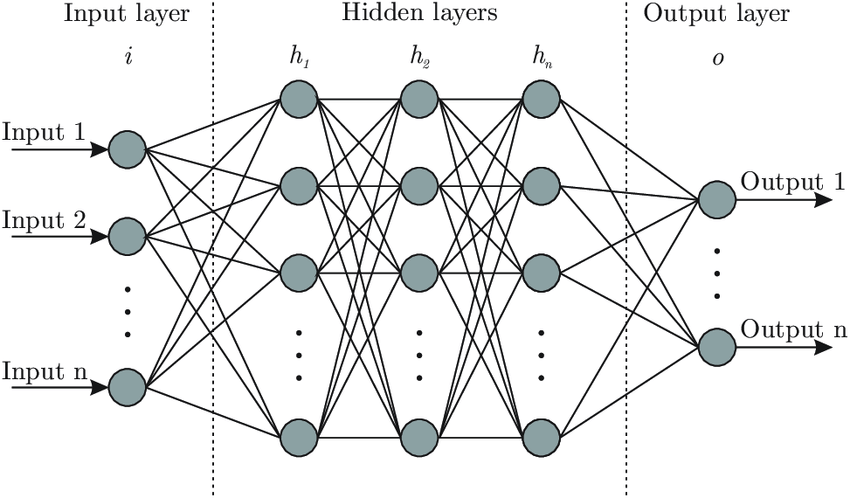
\includegraphics[width=1\textwidth]{THEORETICAL_BACKGROUND/neural_network.png}
    \caption{Γενική μορφή Νευρωνικού δικτύου (Πηγή: \href{https://mc.ai/my-notes-on-neural-networks-2/}{\tl{mc.ai}})}
  \end{center}
\end{figure}

Για την σωστή λειτουργία ενός νευρωνικού δικτύου είναι απαραίτητοι ορισμένοι επιπλέον μηχανισμοί οι οποίοι μετασχηματίζουν τις τιμές εξόδου των κόμβων, αυτές είναι οι συναρτήσεις ενεργοποίησης κάποιες από τις οποίες θα παρουσιαστούν παρακάτω.

\subsection{Ανορθωμένη γραμμική συνάρτηση \tl{(ReLU)}}
Η ανορθωμένη γραμμική συνάρτηση \tl{ReLU (Rectified Linear Unit)} είναι ουσιαστικά η γραμμική συνάρτηση $\mathit{\mathbf{f\left(x\right) = x}}$, η οποία είναι τροποποιημένη στο μέρος της αρνητικής εισόδου της ώστε να μηδενίζει την έξοδο. Η χρήση της είναι συνήθης στην δομή των νευρωνικών δικτύων ως συνάρτηση ενεργοποίησης, λόγω της ιδιότητας της να αποκόπτει αρνητικές τιμές κατά την διάδοση των σημάτων μεταξύ των κόμβων--νευρώνων, κάτι που επιτρέπει την ομαλή εκπαίδευση του.

\begin{figure}[H]
  \begin{center}
    \includesvg[width=1\textwidth]{THEORETICAL_BACKGROUND/ReLU}
    \caption{Μορφή της συνάρτησης ανορθωμένης γραμμικής συνάρτησης \tl{ReLU}}
  \end{center}
\end{figure}

\section{Συνελικτικά Νευρωνικά Δίκτυα}
Τα Συνελικτικά Νευρωνικά Δίκτυα αποτελούν μια συγκεκριμένη μορφή των νευρωνικών δικτύων τα οποία περιλαμβάνουν επίπεδα στα οποία οι κόμβοι δεν είναι πλήρως συνδεδεμένοι με κάθε κόμβο του επομένου επιπέδου αλλά είναι μόνο με ορισμένους που ανήκουν σε μια περιοχή. 

Επίσης χρησιμοποιούνται ορισμένοι ακόμη τύποι επιπέδων όπως για παράδειγμα την τροποποίηση των διαστάσεων της εισόδου με συγκέντρωση μεγίστων (\tl{\textbf{Max Pooling}})

\subsection{Δισδιάστατα Συνελικτικά Επίπεδα}
Τα συνελικτικά επίπεδα είναι το χαρακτηριστικό μέρος των συνελικτικών δικτύων, όπως προδίδει το όνομα τους αποτελούν τμήματα τα οποία μετασχηματίζουν και εξάγουν από την είσοδο πληροφορία με βάση την εφαρμογή συνελικτικών φίλτρων. Η διαδικασία αυτή επιτρέπει την εξαγωγή χρήσιμης πληροφορίας προς τα επόμενα επίπεδα για την ανίχνευση πιθανών μοτίβων ενώ ταυτόχρονα δεν απαιτεί το μέγεθος των πυκνών \tl{dense} επιπέδων καθώς αφορά πράξεις ενός σημείου της εισόδου με ορισμένα γειτονικά σημεία και όχι την μέθοδο πράξεων σημεία όλα προς όλα.

Η μορφή της περιοχής των γειτονικών σημείων καθορίζεται από το φίλτρο \tl{\textbf{Kernel}} που χρησιμοποιείται. Ο πυρήνας που χρησιμοποιείται συνήθως σε δισδιάστατα νευρωνικά δίκτυα είναι διαστάσεων $3\times3$. Ορισμένες ακόμη παράμετροι των πυρήνων είναι ο αριθμός των φίλτρων που υπάρχουν στο συγκεκριμένο επίπεδο αλλά και ο τρόπος που εφαρμόζονται τα συνελικτικά φίλτρα. Η πρώτη παράμετρος είναι το βήμα συνέλιξης ως προς τις 2 διαστάσεις, το οποίο συνήθως είναι μονάδα όπως και εφαρμόστηκε, για τιμές μεγαλύτερες της μονάδας υπάρχει υποδειγματοληψία για το επόμενο επίπεδο. Επίσης κατά την εφαρμογή συνελικτικών φίλτρων υπάρχει η επιλογή συνέλιξης στα άκρα του δισδιάστατου επιπέδου με μέχρι 

Κατά την εφαρμογή ενός συνελικτικού επιπέδου στην είσοδο ή οποιοδήποτε ενδιάμεσο επίπεδο, κάθε συνελικτικό φίλτρο εφαρμόζεται σε όλη την έκταση της εικόνας σύμφωνα με τις παραμέτρους βήματος και την επιλογή για τα ακραία σημεία της εικόνας. Το αποτέλεσμα είναι μια εικόνα ίσων ή μικρότερων διαστάσεων και αριθμού καναλιών $\mathbf{N\times M}$ όπου $\mathbf{N}$ ο αριθμός των καναλιών της εικόνας εισόδου και $\mathbf{M}$ ο αριθμός των φίλτρων του συνελικτικού επιπέδου. Ο αριθμός των παραμέτρων εκπαίδευσης του συνελικτικού επιπέδου είναι ίσος με $\mathbf{\left(A \times B\times N+1\right)\times M}$ όπου $\mathbf{A}$ και $\mathbf{B}$ το πλάτος και ύψος του κάθε συνελικτικού φίλτρου.

Στην υλοποίηση που εξετάζεται χρησιμοποιούνται συνελικτικά επίπεδα 2 διαστάσεων καθώς η είσοδος του δικτύου όπως θα αναφερθεί προκύπτει ως εικόνα ενός καναλιού έπειτα από μετασχηματισμό του αρχικού σήματος.

\subsection{Πλήρως συνδεδεμένα επίπεδα}
Η χρήση των πλήρως συνδεδεμένων επιπέδων είναι απαραίτητη για την αποτελεσματική πρόβλεψη ενός συνελικτικού νευρωνικού δικτύου. Η τοποθέτηση τους στην δομή του μοντέλου ωστόσο προτιμάται να γίνεται σε σημεία όπου η διαστάσεις του προηγούμενου επιπέδου είναι σχετικά μικρές και η επεξεργασία του συγκεκριμένου επιπέδου αφορά την εκτίμηση της προηγουμένως επεξεργασμένης εισόδου.

Στην αρχιτεκτονική των νευρωνικών δικτύων που πραγματεύεται η παρούσα εργασία τα πλήρως συνδεδεμένα επίπεδα τοποθετούνται μετά από τα συνελικτικά επίπεδα και ακριβώς πριν την έξοδο.

\subsection{Επίπεδα υποδειγματοληψίας --- Συγκέντρωση μεγίστων \tl{(Max Pooling)}}
Τα επίπεδα υποδειγματοληψίας είναι σημαντικά για τη δομή ενός συνελικτικού νευρωνικού δικτύου καθώς μειώνουν τις διαστάσεις την διάσταση της εισόδου μειώνοντας έτσι τον αριθμό των παραμέτρων του νευρωνικού δικτύου. Ταυτόχρονα η πληροφορία από τα σημεία της εισόδου που έχουν ενεργοποιηθεί δεν χάνεται. 

Κατά την εφαρμογή ενός επιπέδου συγκέντρωσης ορίζεται μια περιοχή συγκέντρωσης από τις τιμές της εισόδου σε αυτή την περιοχή θα εξαχθεί μια τιμή ανάλογα με τον τύπο επιπέδου συγκέντρωσης. Η διάσταση της περιοχής συγκέντρωσης είναι συνήθως $2\times2$. 

\begin{figure}[H]
  \begin{center}
    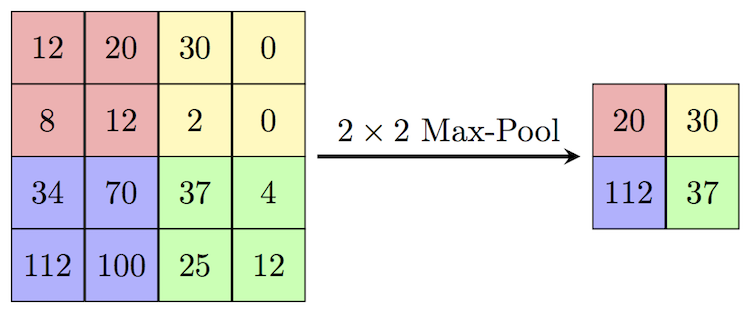
\includegraphics[width=1\textwidth]{THEORETICAL_BACKGROUND/max_pooling.png}
    \caption{Μέθοδος συγκέντρωσης μεγίστων για περιοχές διαστάσεων $2\times2$ (Πηγή: \href{https://computersciencewiki.org/index.php/Max-pooling_/_Pooling}{\tl{Computer Science Wiki}})}
  \end{center}
\end{figure}

Οι 2 τύποι επιπέδων υποδειγματοληψίας είναι η τα συγκέντρωσης μεγίστων και συγκέντρωσης μέσης τιμής. Στην υλοποίηση που χρησιμοποιήθηκε παρατηρήθηκε πως η χρήση συγκέντρωσης μεγίστων έχει σημαντικά καλύτερη επίδοση σε σχέση με την συγκέντρωση μέσου όρου.

\subsection{Αρχικοποίηση Νευρωνικών Δικτύων}
Κατά την αρχικοποίηση ενός νευρωνικού δικτύου, η εκχώρηση των κατάλληλων βαρών των τεχνητών νευρώνων κάθε κόμβου παίζει σημαντικό ρόλο στην μετέπειτα δυνατότητα του μοντέλου να έχει μια στατιστικά αμερόληπτη κατάσταση εκκίνησης της εκπαίδευσης του, έτσι είναι εφικτό να τροποποιούνται τα βάρη του με κατάλληλο τρόπο ώστε να βελτιώνεται η απόδοση του κατά την διαδικασία της εκπαίδευσης.
Για τον παραπάνω σκοπό υπάρχουν ορισμένες μέθοδοι αρχικοποίησης των βαρών ενός μοντέλου
Κατά την πρώτη υλοποίηση χρησιμοποιήθηκε ο αρχικοποιητής των \tl{kernel *random\_uniform*}

\subsection{Μέθοδοί ελαχιστοποίησης σφάλματος --- Βελτιστοποιητές \tl{(Optimizers)}}

Η πιο γνωστή μέθοδος ελαχιστοποίησης σφάλματος είναι η στοχαστική κατάβαση δυναμικού \tl{\textbf{SGD (Stochastic Gradient Descent)}}
Μια από τις μεθόδους ελαχιστοποίησης σφάλματος η οποία παρατηρήθηκε πως είναι κατάλληλη για την χρήση σε συνελικτικά νευρωνικά δίκτυα είναι ο βελτιστοποιητής \tl{Adam}. ...
Ένας ακόμη βελτιστοποιητής που χρησιμοποιείται είναι ο \tl{Nadam} ο οποίος πρόκειται για μια τροποποίηση του \tl{Adam} που συνδυάζει τον βελτιστοποιητή \tl{NAG (Nesterov accelerated SGD)}


\section{Μέθοδος εξαγωγής \tl{Spectrogram}}

\subsection{\tl{Absorbances-Savintzky Golay}}


\section{Μετρικές αξιολόγησης}
$RMSE$, ${R^2}$, $RPIQ$ 

\section{Μετρικές εκπαίδευσης}
\tl{Mean Square Error}
